\section{Problem 2}

\subsection{Identification of the type of filter}

The circuit is a two stages filter. The first stage is a first-order high-pass filter, a single RC with a non-inverting OpAmp for buffering and gain. The second stage is a second-order Sallen-Key low-pass filter. Thus, the circuit, shown in Figure \ref{fig:sch_ex2}, is a third-order pass band filter as a whole. 

\begin{figure}[H]
    \centering
    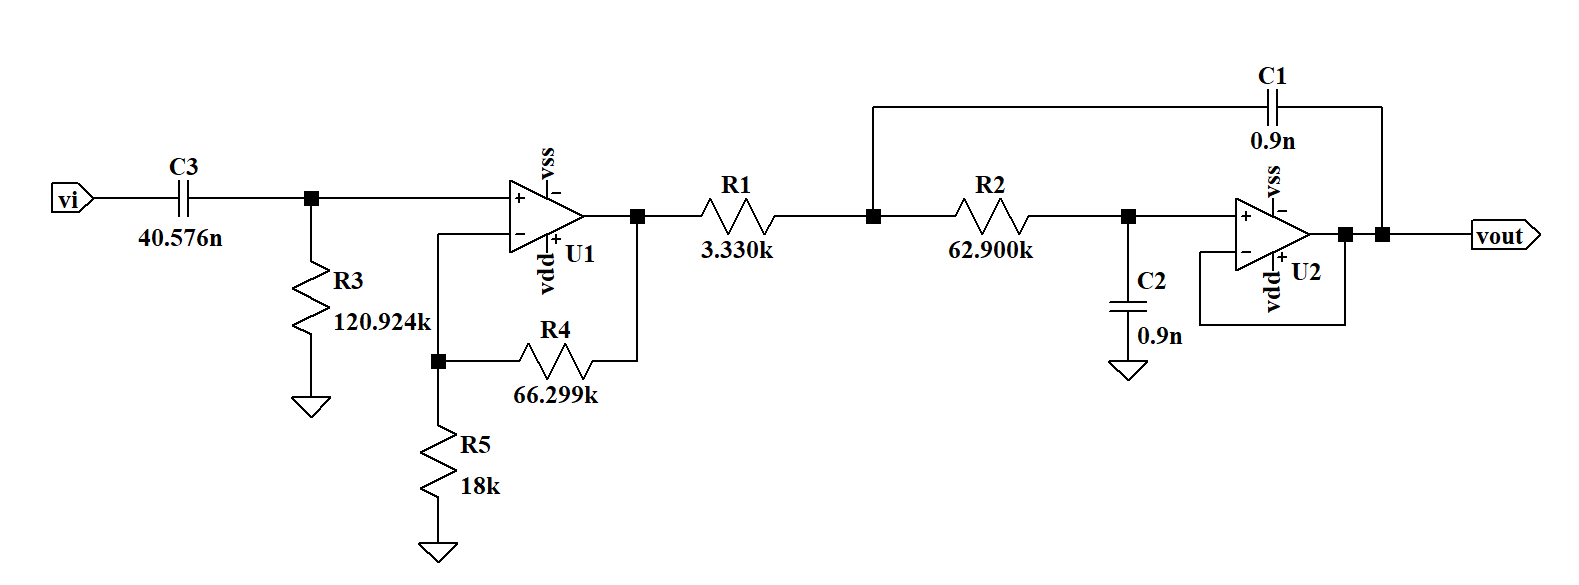
\includegraphics[width=1\linewidth]{images/sch_ex2.png}
    \caption{Circuit schematic of the third-order low-pass filter.}
    \label{fig:sch_ex2}
\end{figure}

\begin{table}[h]
    \centering
    \caption{Element values of the circuit.}
    \begin{tabularx}{\textwidth}{>{\centering\arraybackslash}X >{\centering\arraybackslash}X}
        \toprule
        \textbf{Element} & \textbf{Value}\\
        \midrule
        $R1$ & $3.33k\Omega$\\ \midrule
        $R2$ &  $62.9k\Omega$ \\ \midrule
        $R3$ & $120.92k\Omega$ \\ \midrule
        $R4$ &  $66.3k\Omega$\\ \midrule
        $C1$ & $0.9nF$ \\ \midrule
        $C2$ & $0.9nF$  \\ \midrule
        $C3$ & $40.57nF$ \\
        \bottomrule
    \end{tabularx}
    \label{tab:elements}
\end{table}

\subsection{Filter characterization}
A Python script was developed to obtain the characteristics of the filter. The script is shown in Listing \ref{lst:ex2_script}.

\lstinputlisting[language=Python, caption={Python script to calculate the filter characteristics.}, label={lst:ex2_script}]{python/ex2.py}

In Table \ref{tab:script_results} are shown the results obtained by the Python script.

\begin{table}[h]
    \centering
    \caption{Python script results.}
    \begin{tabularx}{\textwidth}{>{\centering\arraybackslash}X >{\centering\arraybackslash}X}
        \toprule
        \textbf{Element} & \textbf{Value}\\
        \midrule
        $f_{cL}$ & $32.44\Omega$\\ \midrule
        $f_{cH}$ &  $2811.43\Omega$ \\ \midrule
        $f_{3}$ &  $53104.75\Omega$ \\ \midrule
        $A_{max}$ & $13.31$ \\
        \bottomrule
    \end{tabularx}
    \label{tab:script_results}
\end{table}

The Bode diagram, generated in Python of the filter response is shown in Figure \ref{fig:ex2_bode}. 
\begin{figure}[H]
    \centering
    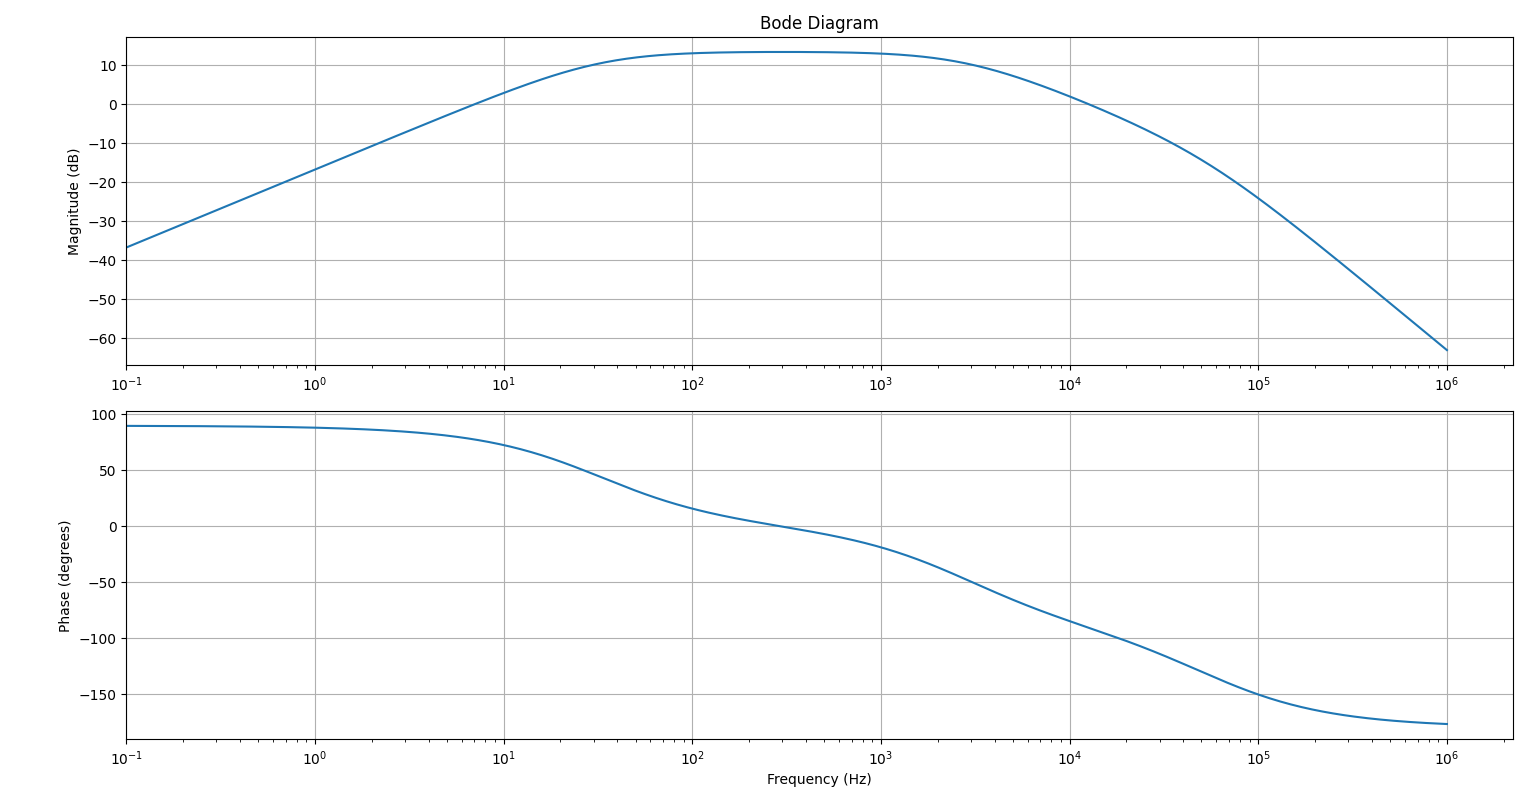
\includegraphics[width=1\linewidth]{images/bode_ex2_python.png}
    \caption{Bode plot of the third-order bandpass filter.}
    \label{fig:ex2_bode_python}
\end{figure}

\subsection{Filter simulation}
In Figure \ref{fig:ex2_bode} is shown the Bode plot of the filter generated in LTSpice. The low cutoff frequency is around $f_{cL} = 30Hz$ and the high cutoff frequency is around $f_{cH} = 3kHz$. The maximum gain at the passband is around $A_{v} = 13.3dB$. The poles frequencies are shown in Table \ref{tab:poles} and compared with the theoretical values. The values obtain from the python script are very close to the simulation values.

\begin{table}[h]
    \centering
    \caption{Poles on simulation and theoretical values.}
    \begin{tabularx}{\textwidth}{>{\centering\arraybackslash}X >{\centering\arraybackslash}X >{\centering\arraybackslash}X}
        \toprule
        \textbf{Poles} & \textbf{Frequency Simulation} & \textbf{Frequency Theoretical}\\
        \midrule
        $p_1$ & $\approx 32.4Hz$ & $32.44 Hz$ \\
        \midrule
        $p_2$ &  $\approx 2.8KHz$ & $2811.43 Hz$ \\
        \midrule
        $p_3$ & $\approx 53KHz$ & $53.104.76 Hz$ \\
        \bottomrule
    \end{tabularx}
    \label{tab:poles}
\end{table}

\begin{figure}[H]
    \centering
    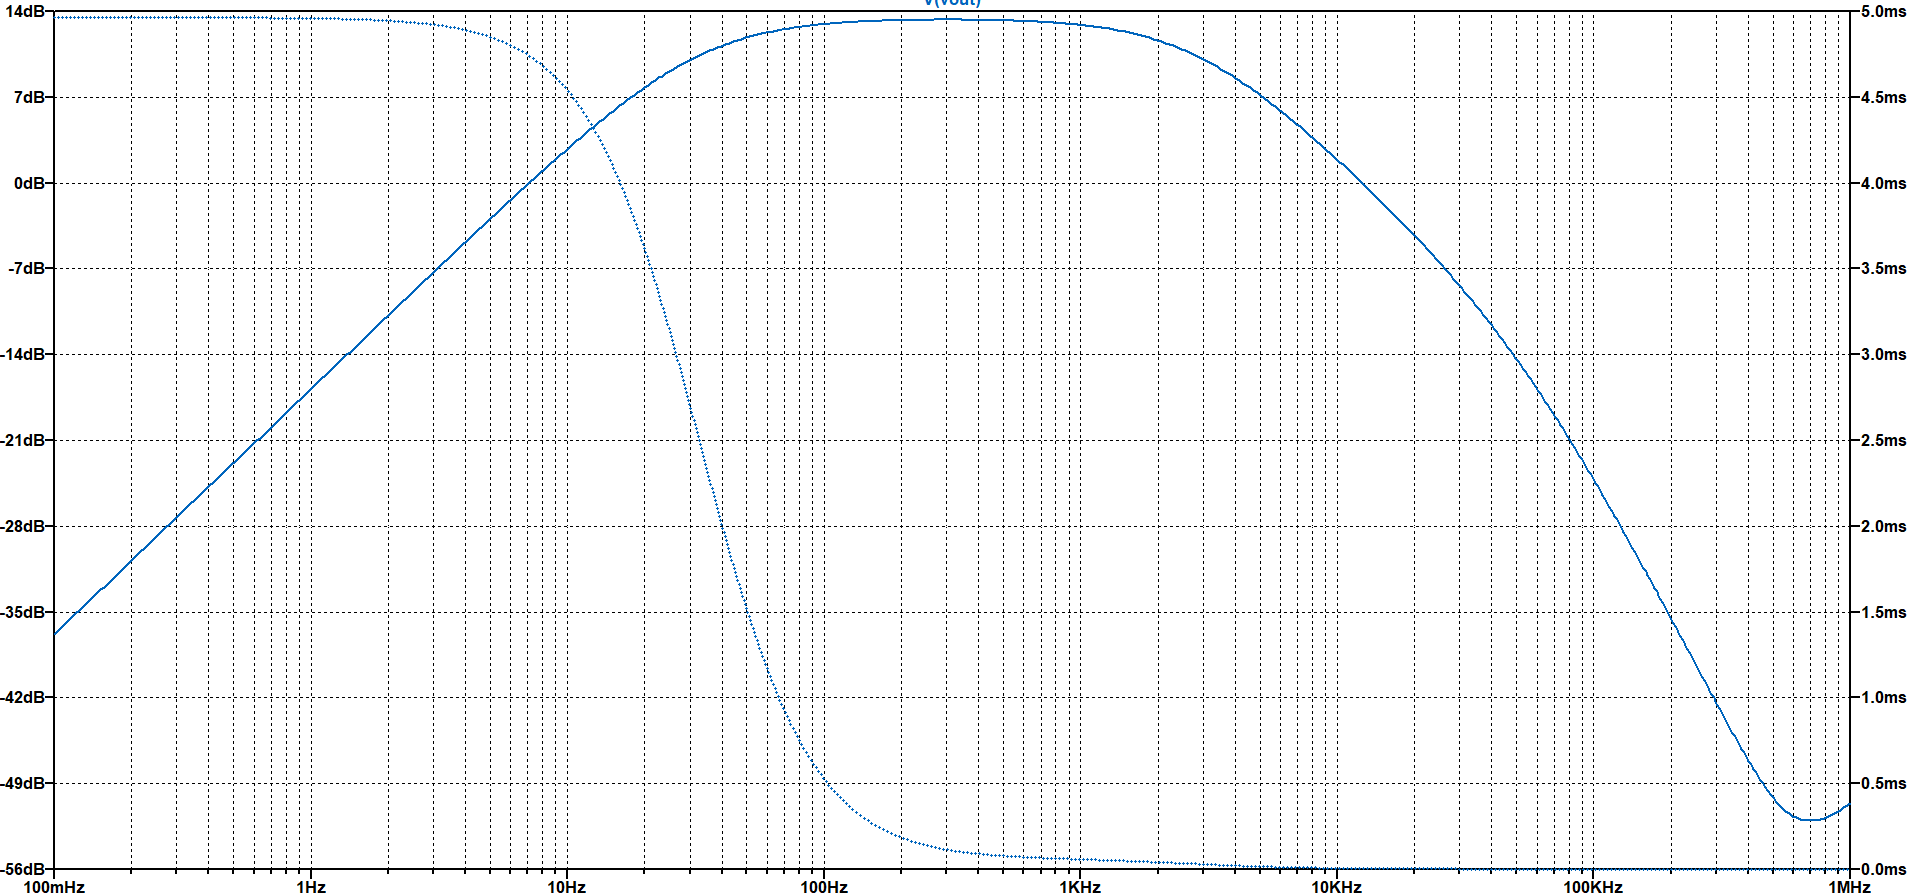
\includegraphics[width=1\linewidth]{images/bode_ex2_ltspice.png}
    \caption{Bode plot of the third-order low-pass filter.}
    \label{fig:ex2_bode}
\end{figure}

Observing the magnitude response at Figure \ref{fig:ex2_bode}, at low frequencies the magnitude rises and stabilizes at a gain around 13.3dB, this corresponds to the passband gain.

The first pole, the low frequency cut-off pole, is responsible for this gain value, the magnitude stabilizes until the next pole, the high frequency cut-off pole, and after that the third pole increases the attenuation value from $20dB/decade$ to $40dB/decade$.

Observing the group delay, it is constant at the passband, which means that the filter does not introduce any phase distortion at the passband.

\begin{figure}[H]
    \centering
    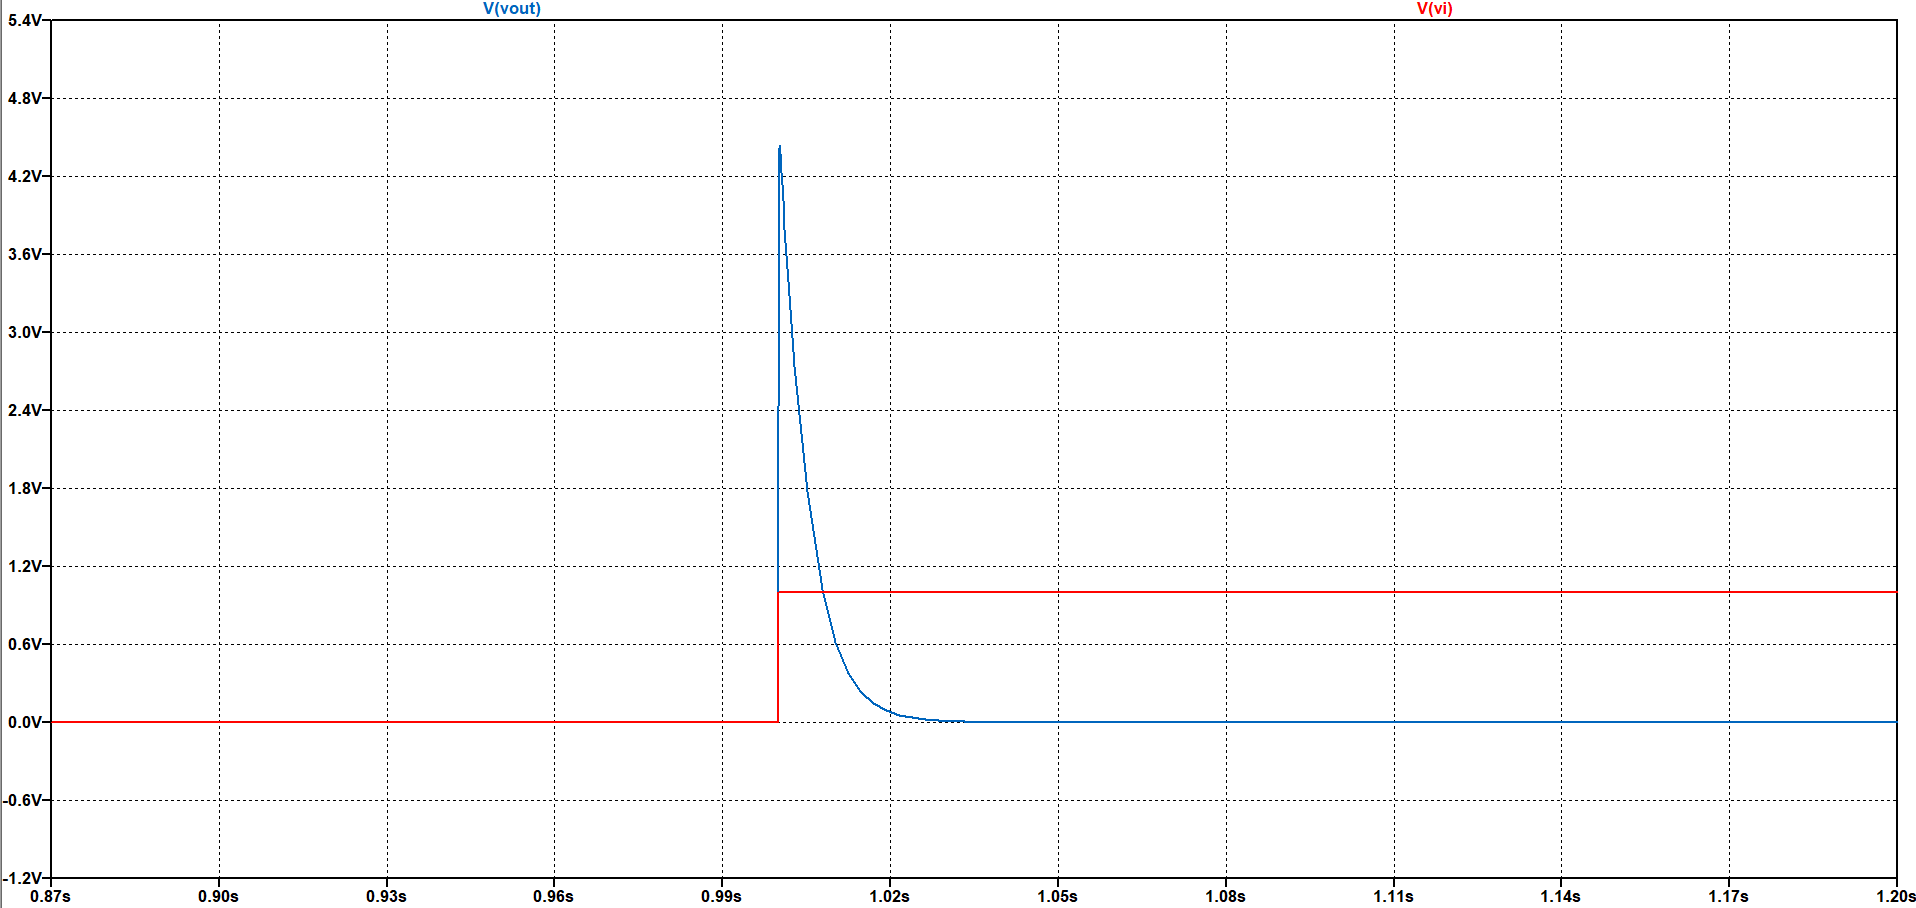
\includegraphics[width=1\linewidth]{images/step_ex2_sim.png}
    \caption{Step response of the third-order low-pass filter.}
    \label{fig:ex2_step}
\end{figure}

In Figure \ref{fig:ex2_step} is represented the step response of the filter. The step response shows that the filter is stable and has a fast response time. When the input step rises, the output shows a sharp initial peak, indicating that the filter reacts strongly to sudden changes in the input signal. The response quickly decays back to zero, the filter ability to reject DC component.

\subsection{Input offset voltages}
\textcolor{red}{Study the impact of the input offset voltages of both OPAMPs. Obtain the expression of the output signal (in the passband region), including the effects of the input offset voltages of both OPAMPs.}

Each OPAMP typically has a small input offset voltage, $V_{OS}$ which is an inherent mismatch in the internal transistors. This causes the OPAMP to behave as if a small DC voltage is applied between its inputs, even when the actual input voltages are equal \textsuperscript{\cite{DC-Parameters-Input-Offset-Voltage}}.

In Figure \ref{fig:sch_vos} is shown the schematic of the filter with the input offset voltages of both OPAMPs.

\begin{figure}[H]
    \centering
    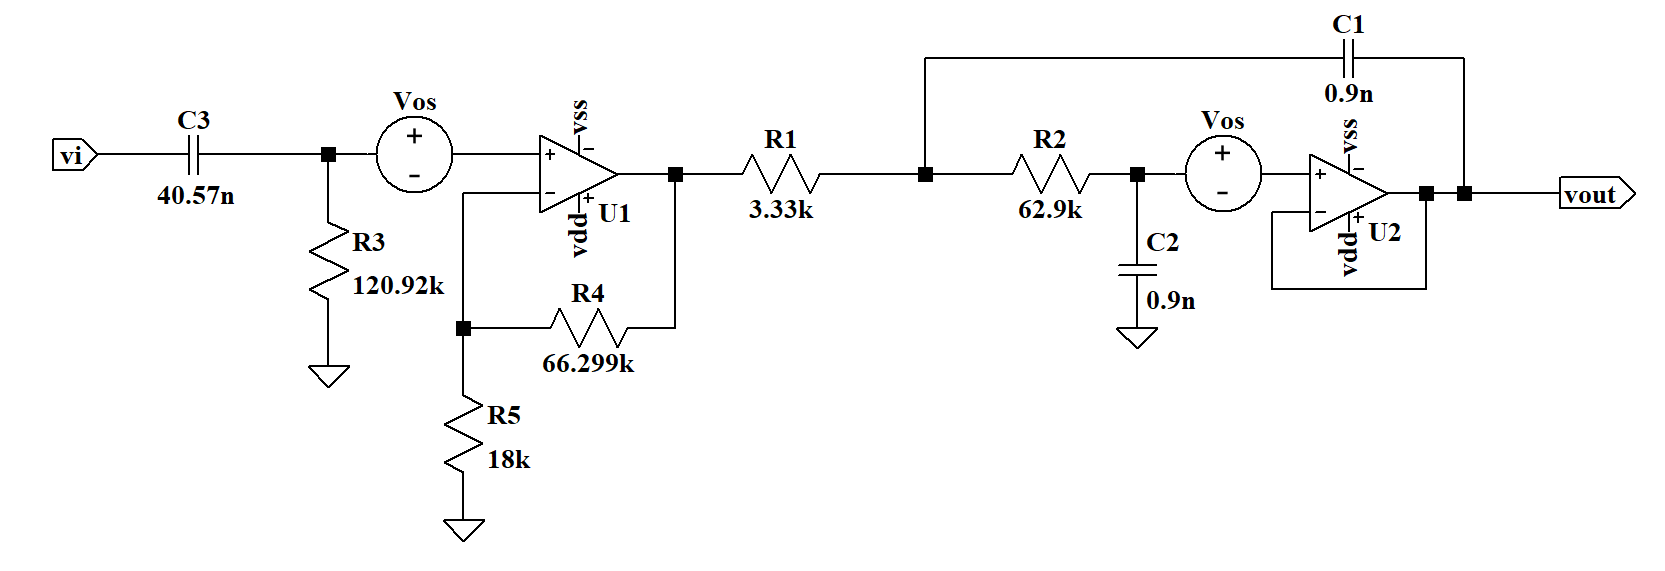
\includegraphics[width=1\linewidth]{images/sch_vos.png}
    \caption{Circuit schematic of the third-order low-pass filter with input offset voltages.}
    \label{fig:sch_vos}
\end{figure}

Analyzing the circuit in Figure \ref{fig:sch_vos}, the output voltage can be calculated using the superposition principle. The output voltage is the sum of the output voltage due to the input offset voltage of the first OPAMP and the output voltage due to the input offset voltage of the second OPAMP. 

como vout é igual à tensão no no no ampop ideal o ofsset será vos

\begin{figure}[H]
    \centering
    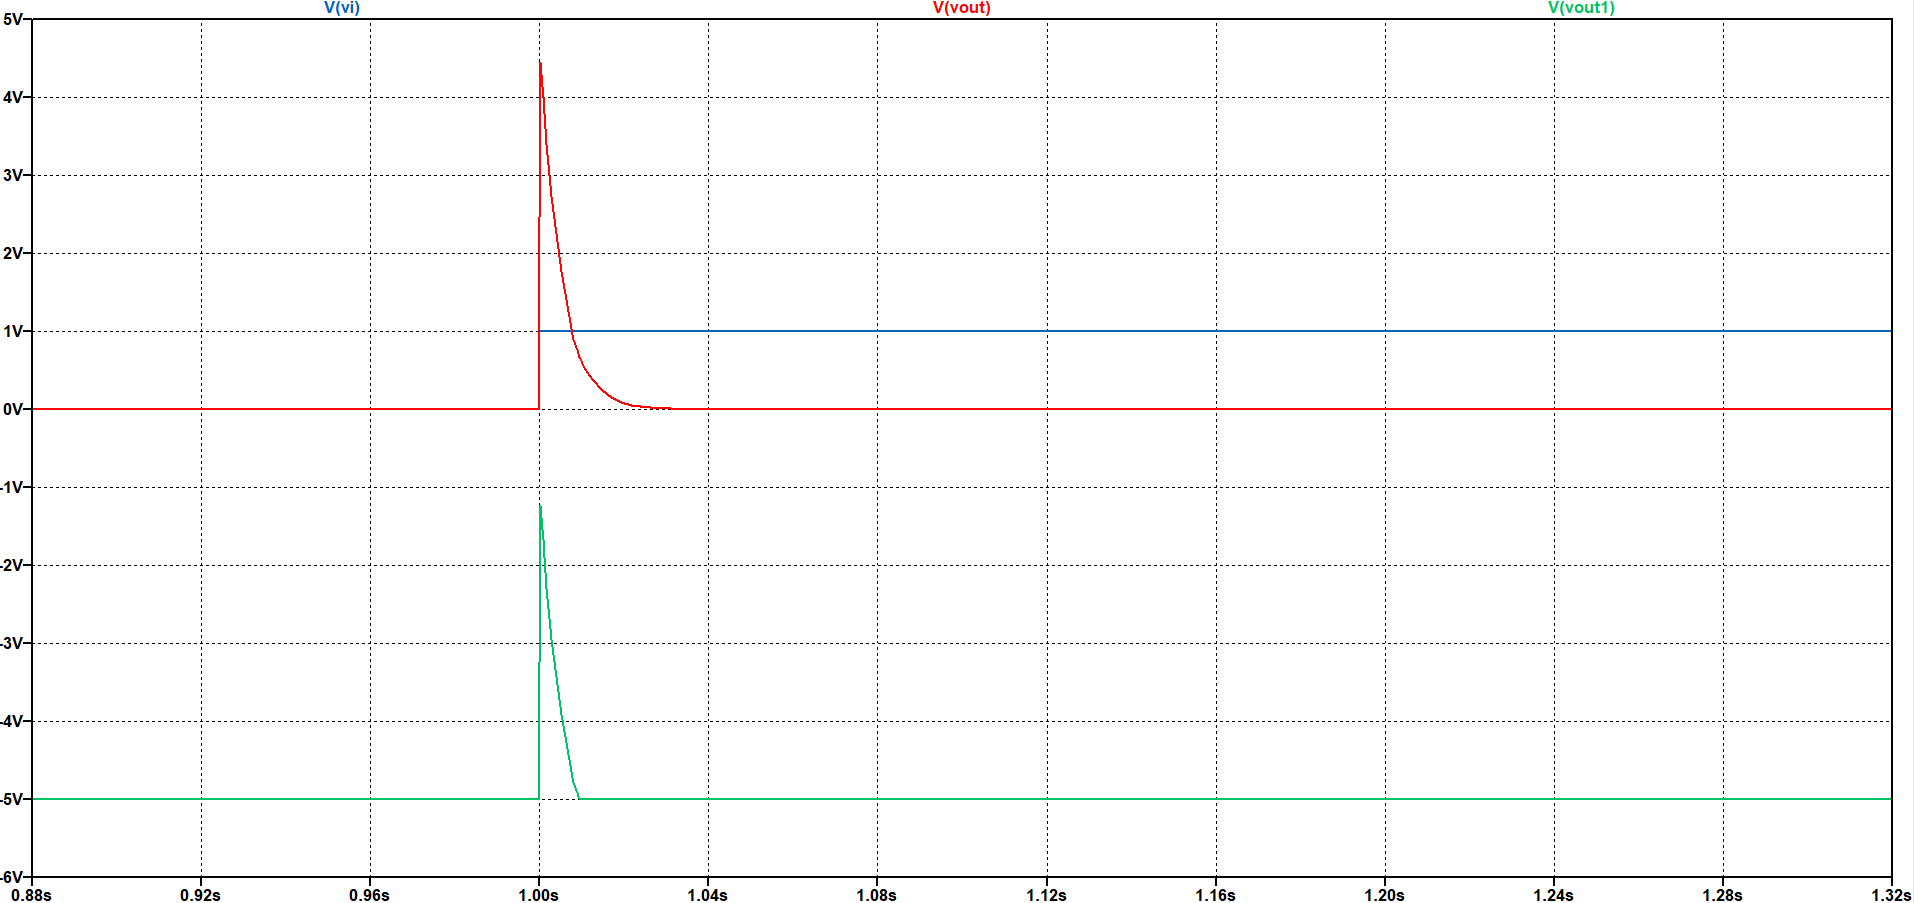
\includegraphics[width=1\linewidth]{images/step_vos.png}
    \caption{Step response of the third-order low-pass filter with input offset voltages.}
    \label{fig:step_vos}
\end{figure}

Observing the step response in Figure \ref{fig:step_vos2}, the input offset voltages cause an offset in the output signal, the output signal is not zero when the input signal is zero. The input offset voltages of both OPAMPs causes a DC offset in the output signal.

\begin{figure}[H]
    \centering
    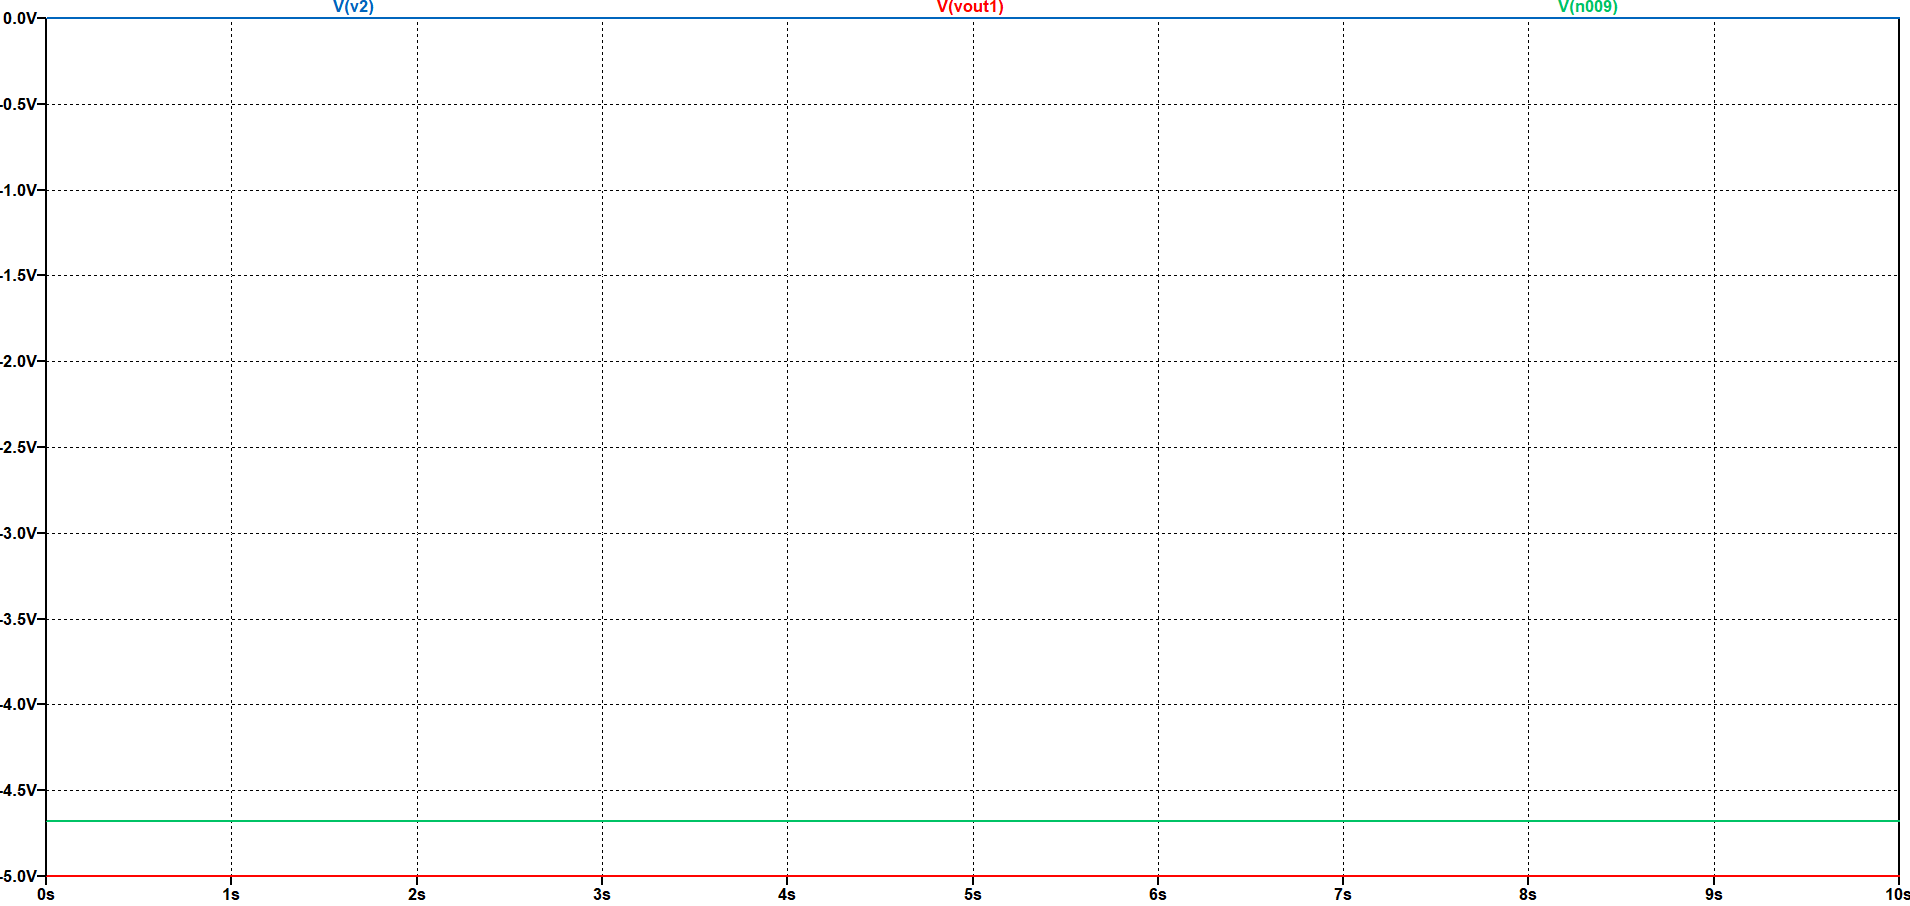
\includegraphics[width=1\linewidth]{images/step_vos2.png}
    \caption{Step response of the third-order low-pass filter with 0V input signal}
    \label{fig:step_vos2}
\end{figure}

\subsection{GBW Specification}
The GBW of an OPAMP defines how its gain decreases with frequency. The closed-loop gain ($A_{v}$) at a particular frequency ($f$) can be calculated using the GBW of the OPAMP and a desired operation frequency, it can be calculated using the following equation \ref{eq:av}:

\begin{equation}
    A_{v} = \frac{GBW}{f}
    \label{eq:av}
\end{equation}

\begin{figure}[H]
    \centering
    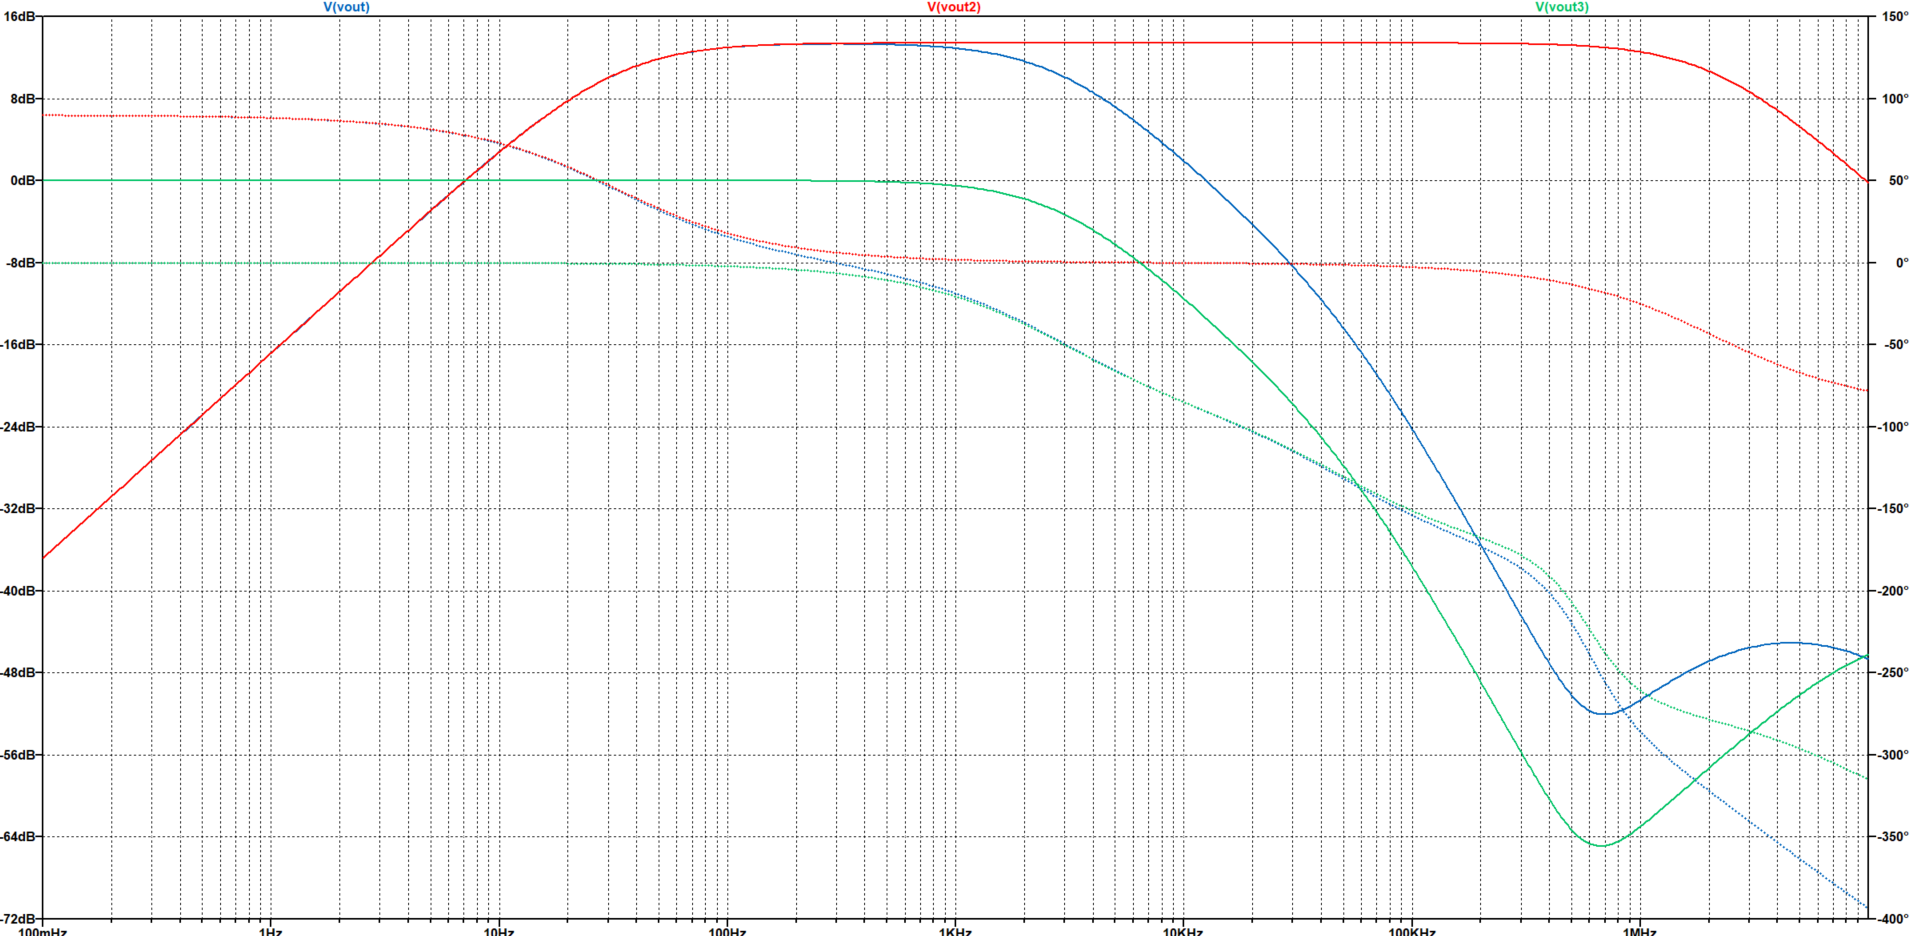
\includegraphics[width=1\linewidth]{images/bode-stages.png}
    \caption{Bode plot of the filter stages and the filter as a whole.}
    \label{fig:bode-stages}
\end{figure}

Observing the Figure \ref{fig:bode-stages}, the gain of the filter is introduced by the first stage of the filter, the second stage is a unity gain buffer. The gain of the first stage is around $13.3dB$. Thus, the first stage needs a higher GBW than the second stage. 

The GBW of the first stage is given by:

\begin{equation}
    GBW = A_v \times f = 10^{(13.3/20)} \times 3kHz = 12.9kHz
\end{equation}

The GBW of the second stage is given by:

\begin{equation}
    GBW = A_v \times f = 1 \times 3kHz = 3kHz
\end{equation}

For this filter, the minimum GBW needed for the OPAMP is 12.9kHz. Hence the OPAMP with a GBW of 10kHz is not adequate for the filter.

\subsection{Rail-to-rail capability}
The maximum signal excursion at the output of an OPAMP is limited. Considering that the
OPAMP has a rail-to-rail capability at the output, determine the maximum input signal
amplitude below which the output does not saturate.

The output voltage of the OPAMP is limited by its power supply voltages:

\begin{equation}
    \begin{aligned}
        V_{out(max)} = V_{cc} - V_{headroom} \\
        V_{out(min)} = V_{ee} + V_{headroom}
    \end{aligned}
\end{equation}

For ideal OPAMPs, the output voltage is limited by the power supply voltages. For real OPAMPs, the output voltage is limited by the headroom voltage, which is the voltage drop between the power supply voltage and the output voltage. 

To determine the output voltage range, the headroom voltage must be considered. 

The output voltage is related to the input voltage by the gain of the OPAMP:

\begin{equation}
    V_{out} = A_v \times V_{in}
\end{equation}

For the output to stay within the output voltage range, the input voltage must be limited by:

\begin{equation}
    -V_{negative-rail} <= A_v \times V_{in} <= V_{positive-rail}
\end{equation}

Thus, the maximum input signal amplitude is given by:

\begin{equation}
    V_{in(max)} = \frac{V_{rail}}{A_v}
\end{equation}

Where $V_{rail}$ is the smaller of the two power supply voltages.

The maximum input signal amplitude is the maximum input signal amplitude that does not saturate the output of the OPAMP.

In this case, the relationship between the $V_{in}$ and $V_rail$ is given by:

\begin{equation}
    V_{in(max)} = \frac{V_{rail}}{10^{(13.3/20)}} = \frac{V_{cc}}{4.62}
\end{equation}

\subsection{OpAmp Selection}
Select a commercial OPAMP that fits the filter specifications. Explain which OPAMP
parameters/criteria were considered in your decision. For example: GBW?, supply voltage?, …,
price?, etc.


\subsubsection{Gain Bandwidth Product (GBW):}

The OPAMP's GBW should be equal or higher than the required GBW for the filter stages. Hence, for a filter that requires a GBW of 12.9 kHz, the choosen OPAMP as to accomplish a GBW of 12.9 kHz or higher.

\subsubsection{Noise Performance:}

The OPAMP's noise performance is crucial for low-noise applications. The input-referred noise voltage should be as low as possible. For instance, if the input-referred noise voltage is $10 nV/\sqrt{Hz}$, the total noise voltage at the output can be calculated as follows:

\begin{equation}
    V_{noise} = \sqrt{f_{BW}} \times V_{n}
\end{equation}

Where $f_{BW}$ is the bandwidth of the filter and $V_{n}$ is the input-referred noise voltage of the OPAMP.

\subsubsection{Slew Rate:}

The slew rate must be high enough to avoid distortion at the maximum signal frequency and amplitude:

\begin{equation}
    Slew Rate \geq 2\pi f_{max} V_{peak}
\end{equation}

\subsubsection{Input Offset Voltage:}

For circuits sensitive to DC biasing errors, the selection of an OPAMP with low input offset voltage is mandatory.

The OPAMP selected was the MCP6002, a dual OPAMP with a GBW of 1 MHz, a slew rate of 0.6 V/$\mu$s, and an input offset voltage of 4 mV. The MCP6002 is a low-power CMOS OPAMP with rail-to-rail input and output. The MCP6002 is a good choice for this filter because it has a GBW higher than the required GBW for the filter stages, a low input offset voltage, and a low price\textsuperscript{\cite{mcp-datasheet}}.

\subsection{Signal to Noise Ratio}
\textcolor{red}{Considered an input sinusoidal input with 10 mV of amplitude and with a frequency inside the
pass band of the filter. Obtain the signal to noise ratio at the output node. Consult the input
referred noise value of the opamp indicated in the moodle page.}

\subsection{Single supply version}
textcolor{red}{Modify the circuit of Figure 2 to operate with only one power supply, i.e., propose a single supply version.}
